\section{Ergebnisse}
Die Zusammenfassung der Ergebnisse ist in \autoref{anh:ergebnisse} zu finden und umfasst vier Tabellen. Die Aufteilung in die vier Tabellen geschah entsprechend der Kompressionsverfahren, das bedeutet eine Tabelle enthält die Ergebnisse aller drei Kompressionsraten, aufgeteilt in die drei Datensätze und in die vier Analyseverfahren. Die ersten vier Werte entsprechen richtig positiv, richtig negativ, falsch positiv und falsch negativ, während die letzten beiden Werte für Sensitivität und Präzision stehen (siehe \autoref{sec:auswertung} für Bedeutungen und Abkürzungen). In dem folgenden Abschnitt sind diese Ergebnisse in vier Abbildungen mit jeweils drei Plots der F$_1$"=Maße aufgeteilt. Die Aufteilung geschah auch hier entsprechend der Kompressionsverfahren, das bedeutet in einer Abbildung findet sich ein Plot je Datensatz. Die x"=Achse eines Plots stellt die Kompressionsrate dar und die y"=Achse das F$_1$"=Maß. Die verschiedenfarbigen Linien zeigen die Entwicklung des F$_1$"=Maßes eines Analyseverfahrens, entlang sinkender Kompressionsrate.


In einem ersten Blick fällt auf, dass die Analyseverfahren zu einem großen Teil gut abschnitten. Dass bedeutet, dass in den meisten Fällen das F$_1$"=Maß über 0,7 lag und somit ein gutes Gleichgewicht zwischen Sensitivität und Präzision herrscht, egal welches Kompressionsverfahren und "=rate. Allerdings gibt es auch äußerst schlechte Ergebnisse, so zum Beispiel in \autoref{subfig:f1polecg}, wo nahezu alle Werte unter 0,5 sind oder die Random Projection sogar dauerhaft F$_1$"=Maße von 0,0 oder leicht darüber hat.

Genau so gibt es aber auch äußerst positive Fälle, wie in \autoref{tab:datakompfour} bei $\rho=0,50$ NVIDIA-Aktie, bei dem egal welches Analyseverfahren 100\% der ursprünglichen Datenpunkte erkannt hat und lediglich die Random Projection fälschlicherweise noch neun weitere Ausreißer erkannt und somit die Präzision bei 80\% liegt.

\begin{figure}[bth]
  \subfloat[Wetterdaten]{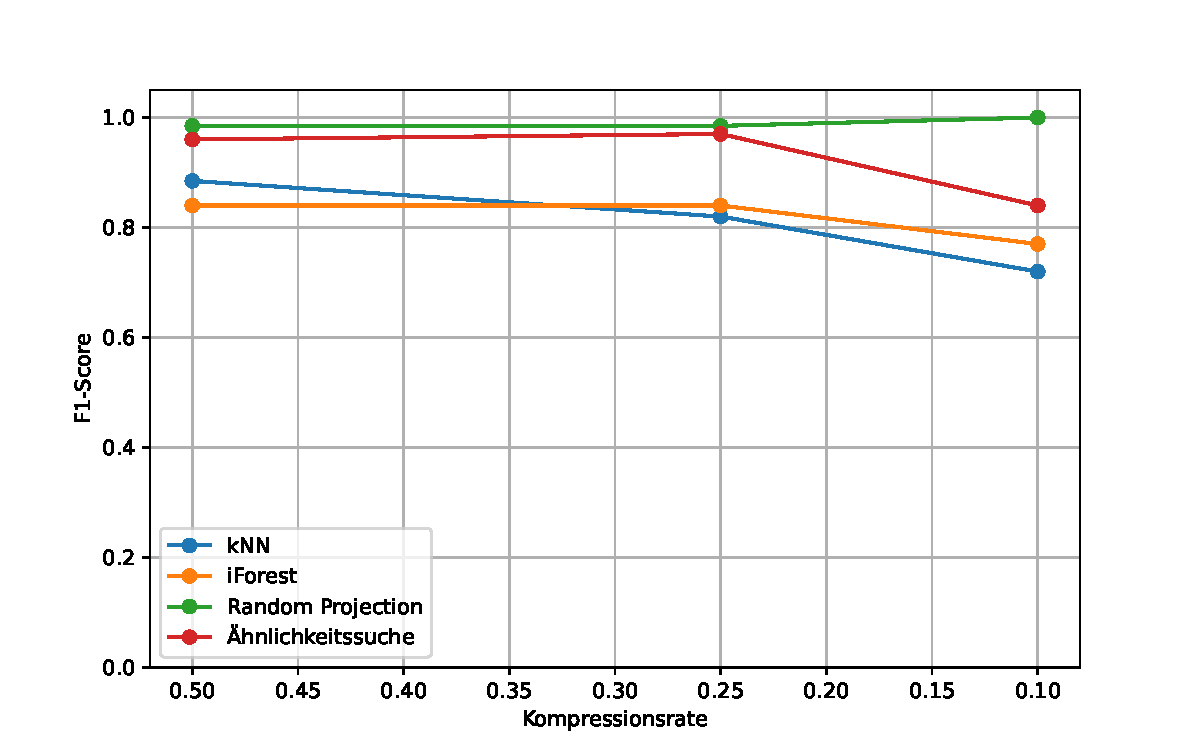
\includegraphics[width=0.49\textwidth]{Graphics/F1LinearWetter.pdf}\label{subfig:f1linwetter}}\hfill
  \subfloat[NVIDIA]{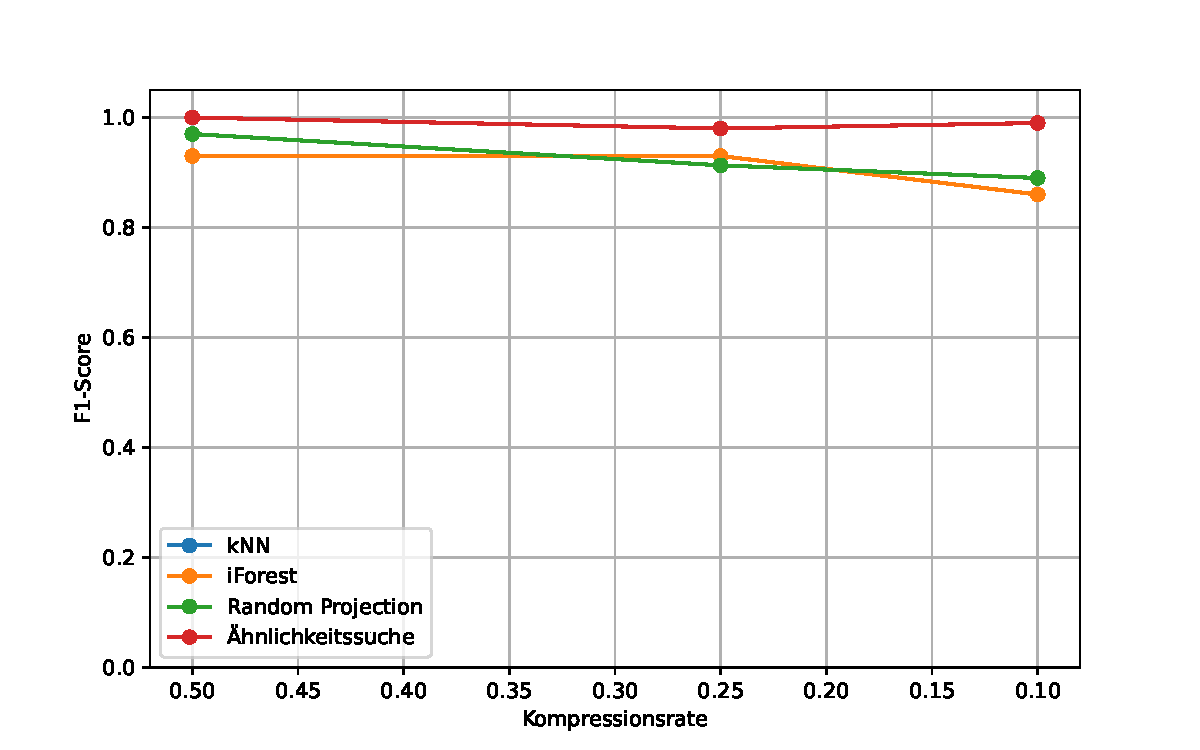
\includegraphics[width=0.49\textwidth]{Graphics/F1LinearNvidia.pdf}\label{subfig:f1linnvidia}}\hfill
  \centering\subfloat[ECG5000]{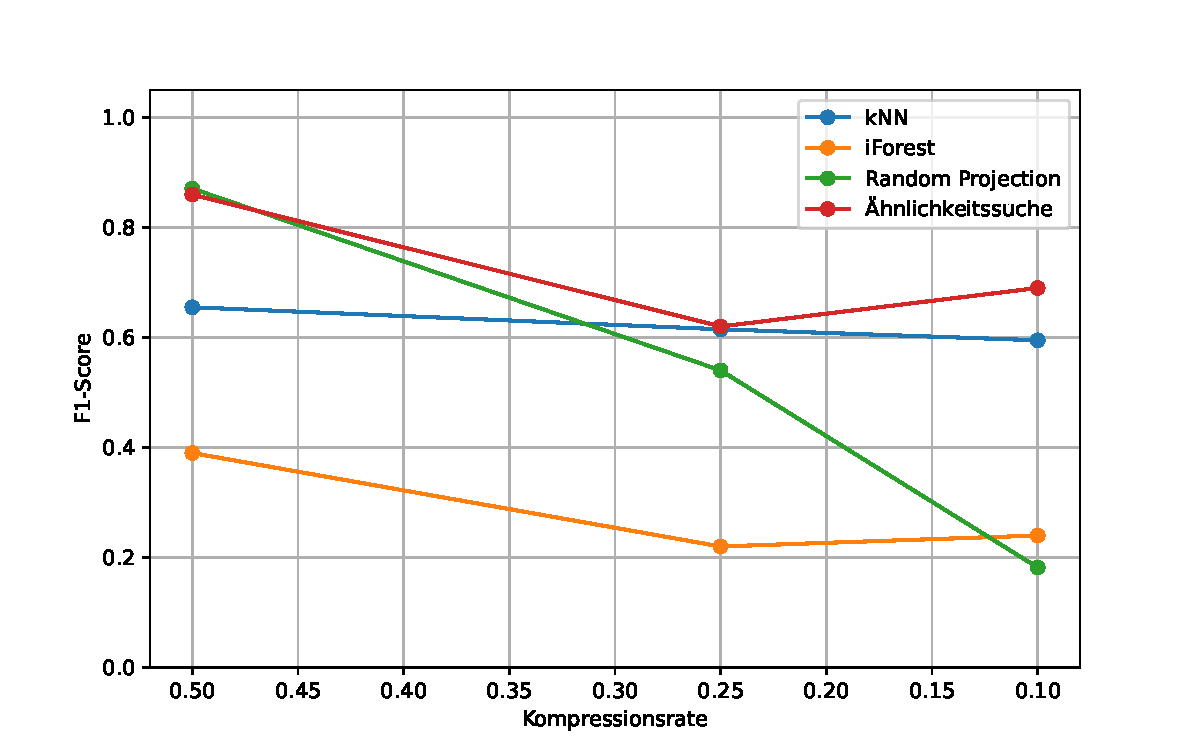
\includegraphics[width=0.49\textwidth]{Graphics/F1LinearECG.pdf}\label{subfig:f1linecg}}
  \caption{F1"=Maße der Analyseverfahren bei linearer Kompression}
  \label{fig:f1LinMaße}
\end{figure}

\begin{figure}[bth]
  \subfloat[Wetterdaten]{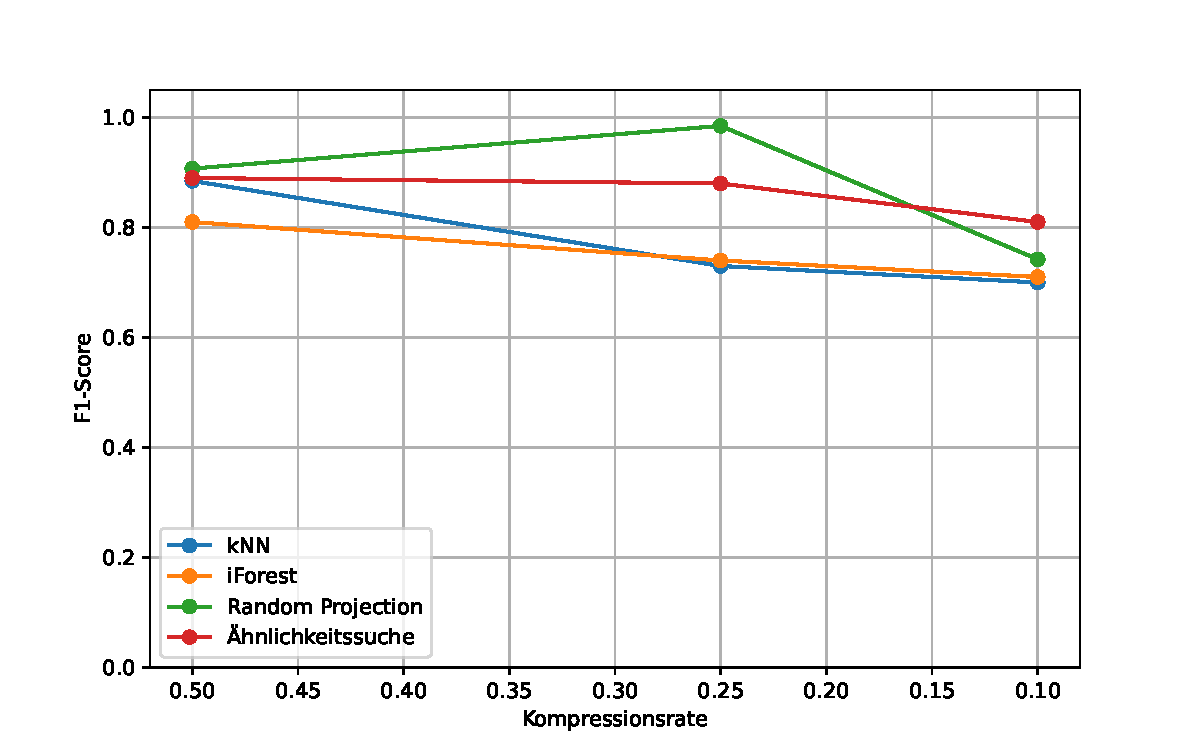
\includegraphics[width=0.49\textwidth]{Graphics/F1PolyWetter.pdf}\label{subfig:f1polwetter}}\hfill
  \subfloat[NVIDIA]{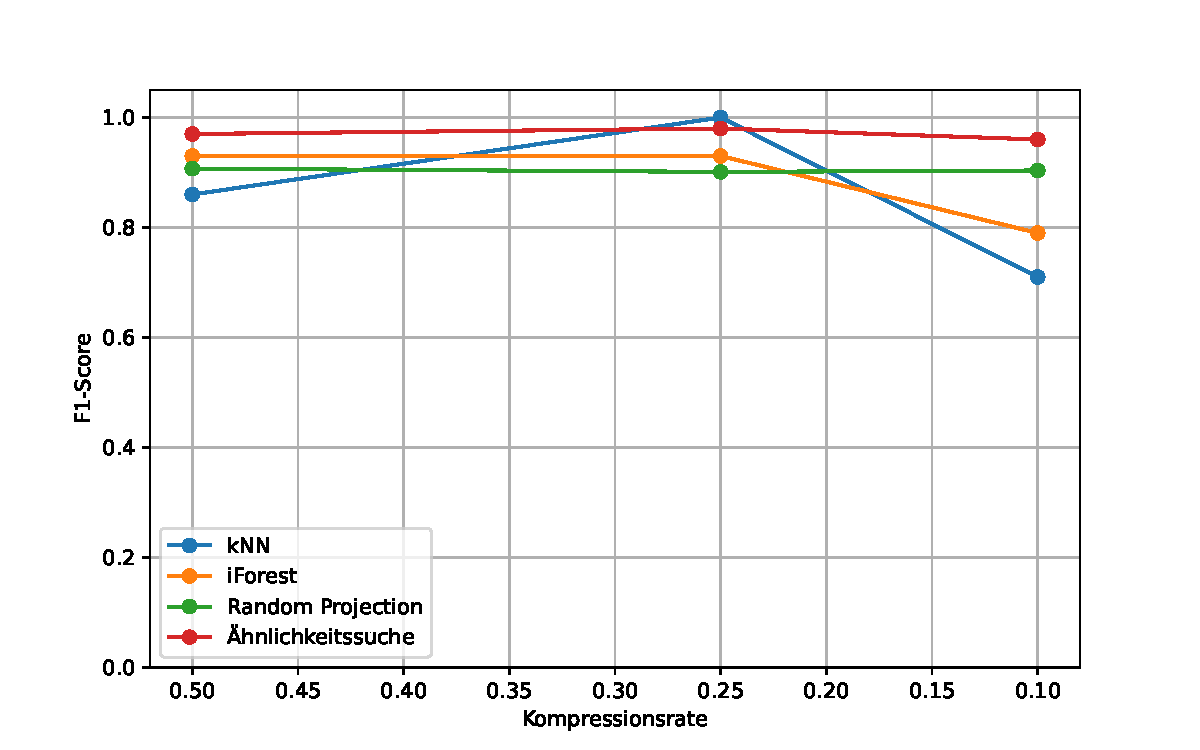
\includegraphics[width=0.49\textwidth]{Graphics/F1PolyNvidia.pdf}\label{subfig:f1polnvidia}}\hfill
  \centering\subfloat[ECG5000]{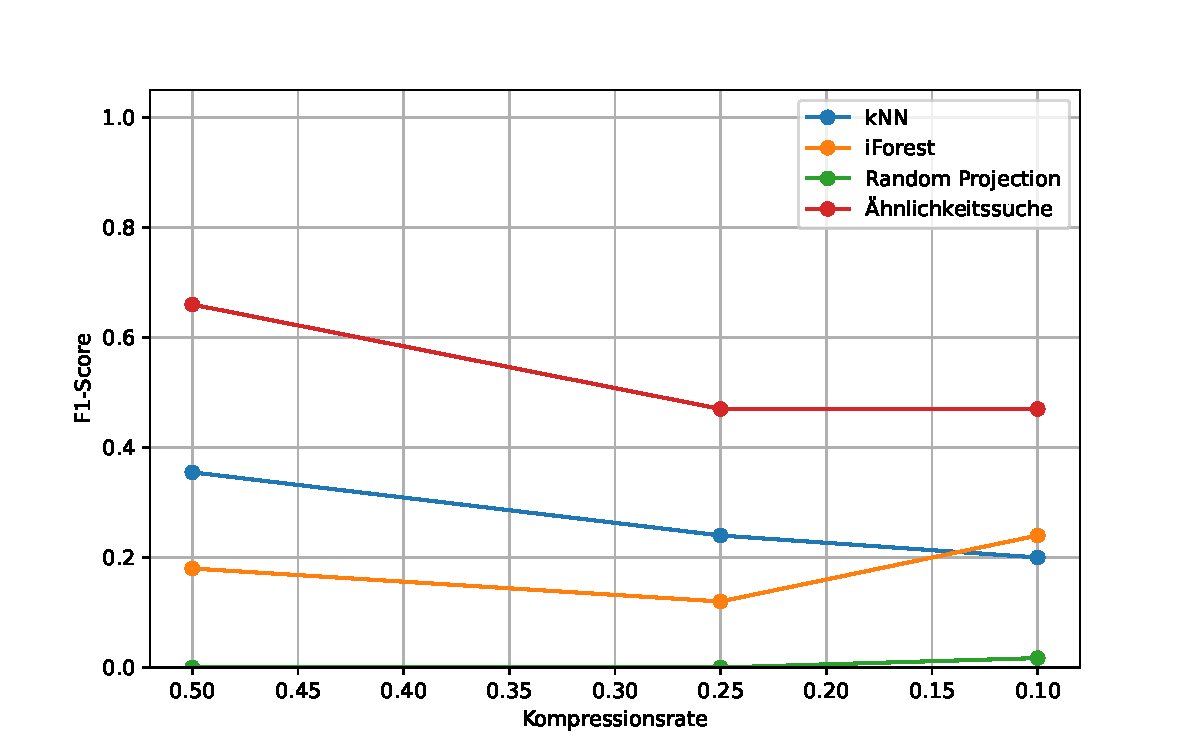
\includegraphics[width=0.49\textwidth]{Graphics/F1PolyECG.pdf}\label{subfig:f1polecg}}
  \caption{F1"=Maße der Analyseverfahren bei polynomieller Kompression}
  \label{fig:f1PolMaße}
\end{figure}

\begin{figure}[bth]
  \subfloat[Wetterdaten]{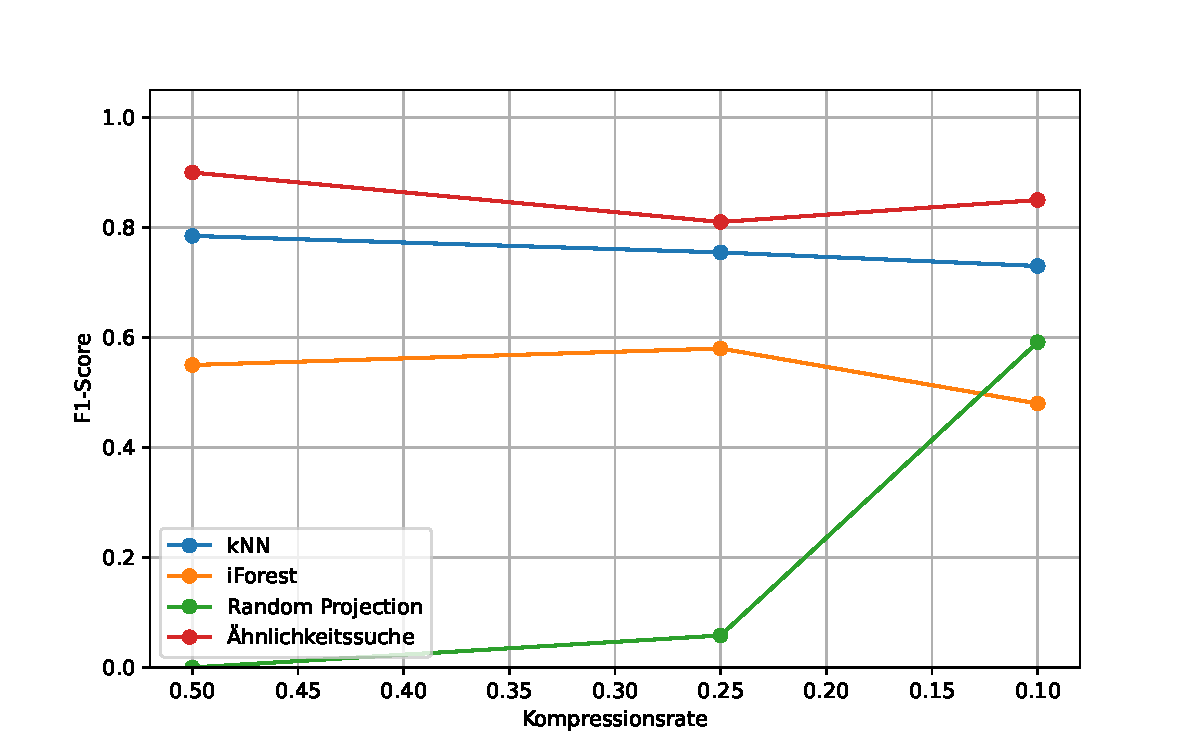
\includegraphics[width=0.49\textwidth]{Graphics/F1FourierWetter.pdf}\label{subfig:f1fourierwetter}}\hfill
  \subfloat[NVIDIA]{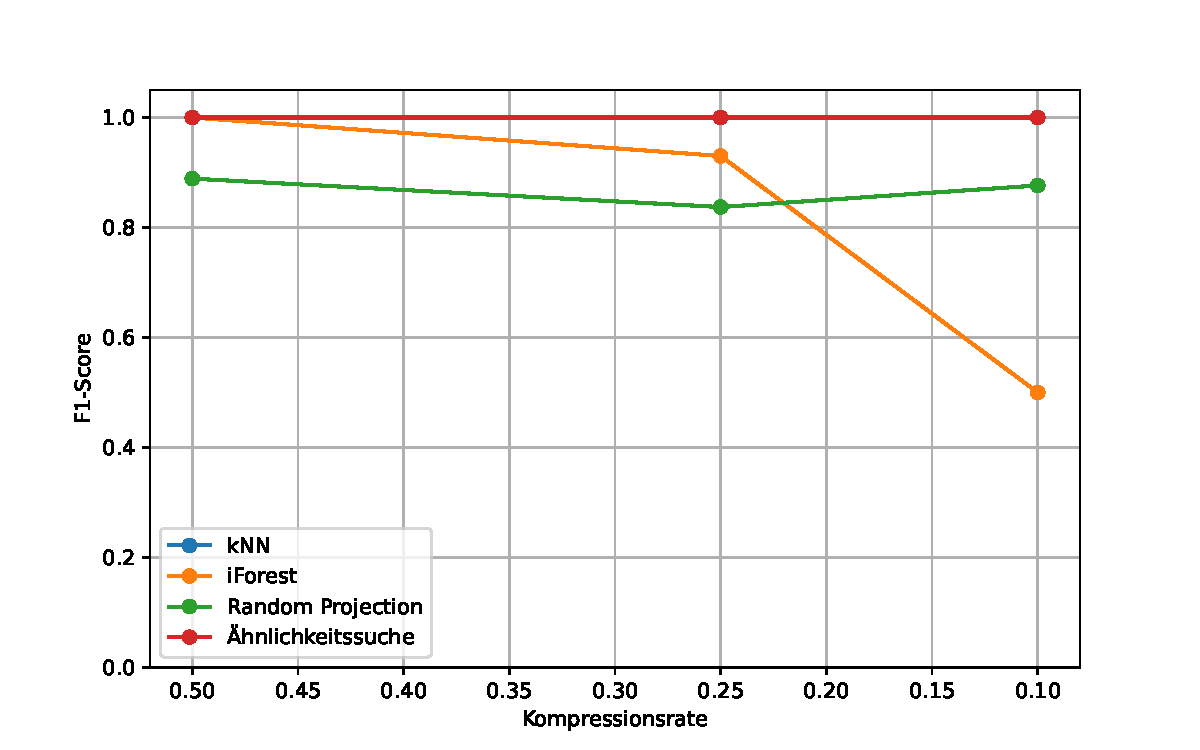
\includegraphics[width=0.49\textwidth]{Graphics/F1FourierNvidia.pdf}\label{subfig:f1fouriernvidia}}\hfill
  \centering\subfloat[ECG5000]{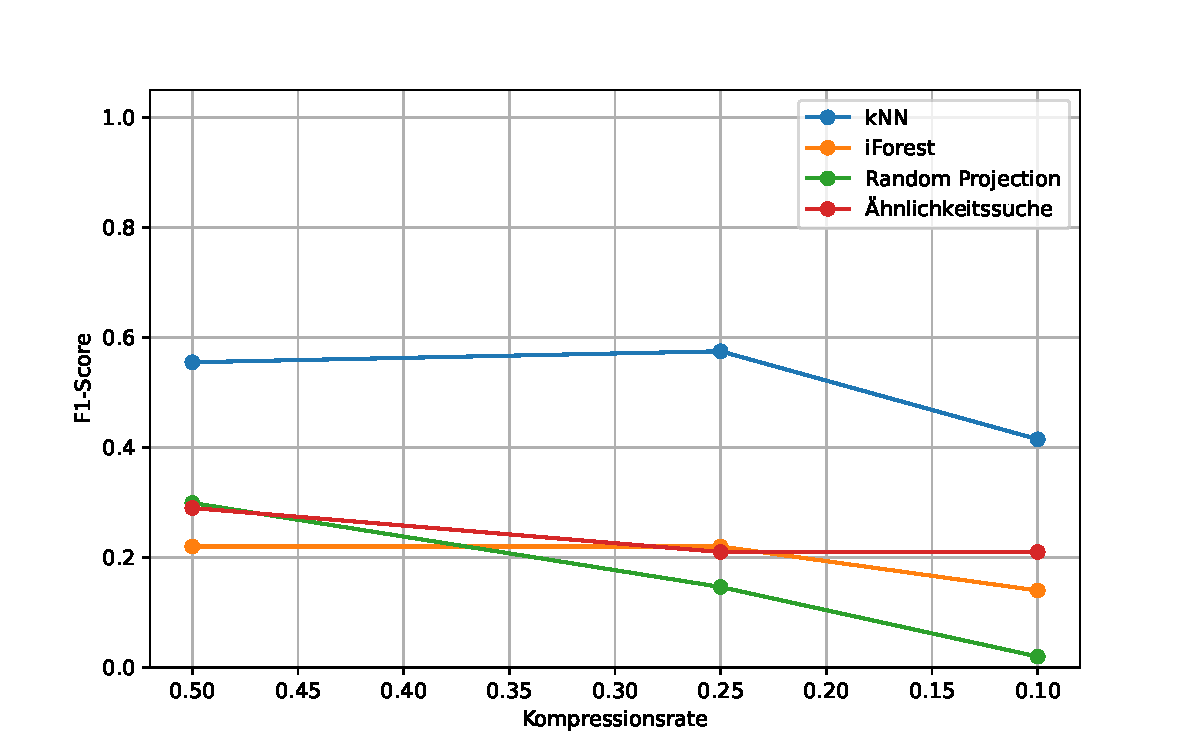
\includegraphics[width=0.49\textwidth]{Graphics/F1FourierECG.pdf}\label{subfig:f1fourierecg}}
  \caption{F1"=Maße der Analyseverfahren bei Fourier"=Kompression}
  \label{fig:f1FourMaße}
\end{figure}

\begin{figure}[bth]
  \subfloat[Wetterdaten]{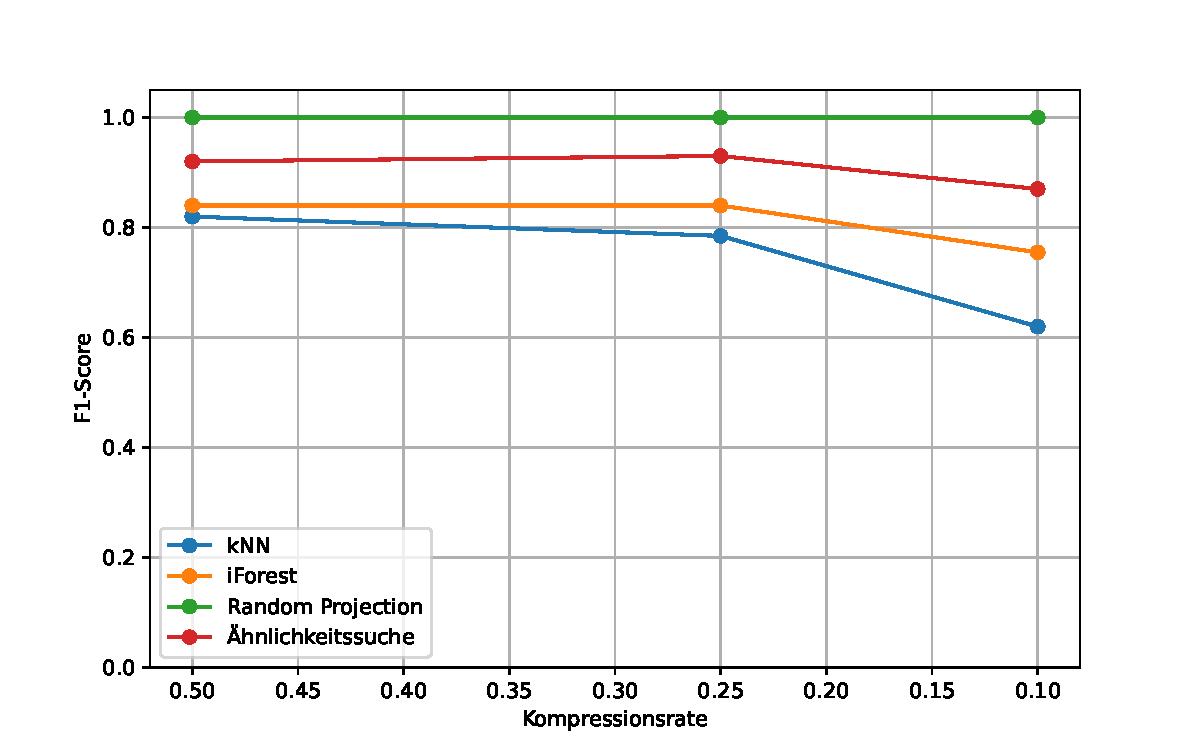
\includegraphics[width=0.49\textwidth]{Graphics/F1WaveletWetter.pdf}\label{subfig:f1waveletwetter}}\hfill
  \subfloat[NVIDIA]{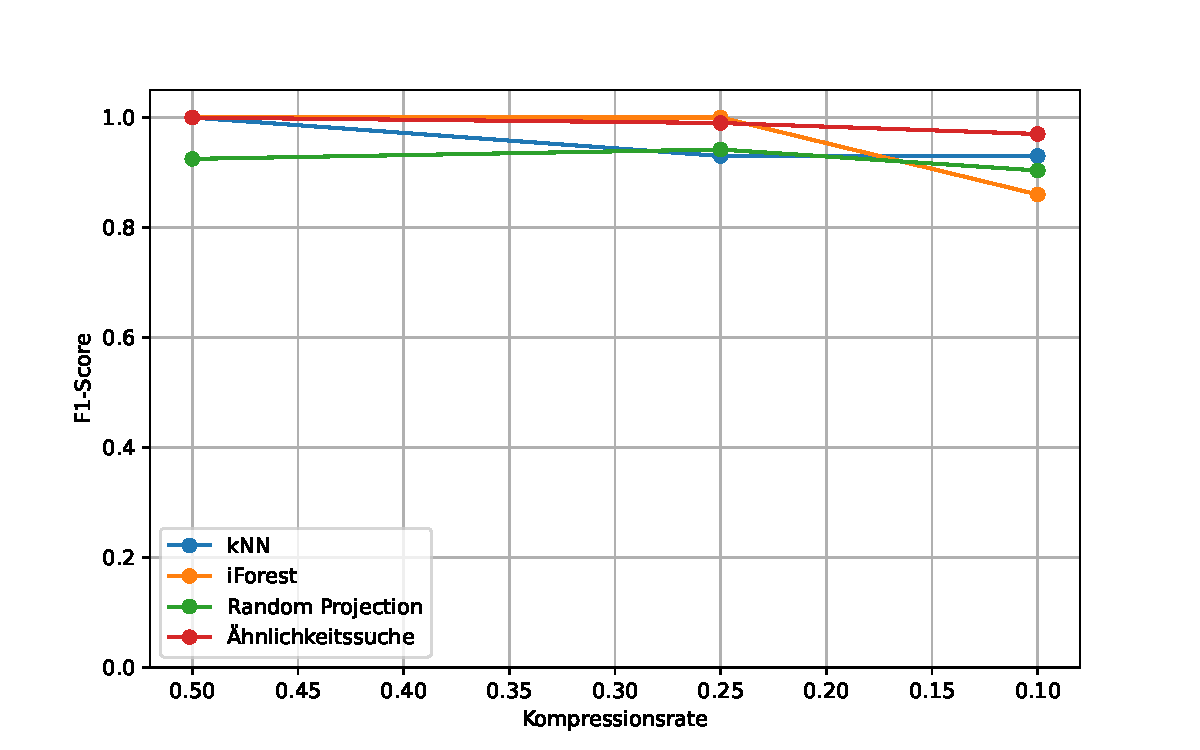
\includegraphics[width=0.49\textwidth]{Graphics/F1WaveletNvidia.pdf}\label{subfig:f1waveletnvidia}}\hfill
  \centering\subfloat[ECG5000]{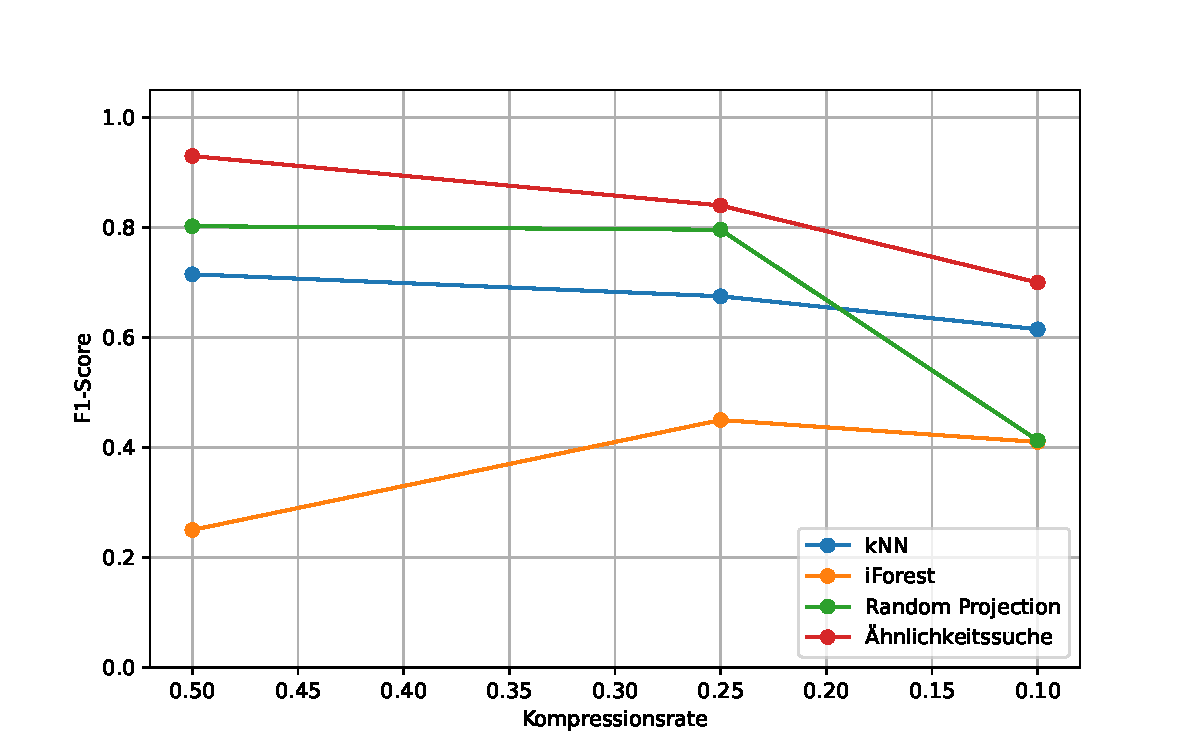
\includegraphics[width=0.49\textwidth]{Graphics/F1WaveletECG.pdf}\label{subfig:f1waveletecg}}
  \caption{F1"=Maße der Analyseverfahren bei Wavelet"=Kompression}
  \label{fig:f1WaveletMaße}
\end{figure}

